% Skip over this boring header down a bit
%%%%%%%%%%%%%%%%%%%%%%%%%%%%%%%%%%%%%%%%%%%%%%%%
\documentclass[usenames,dvipsnames,10pt,aspectratio=169]{beamer} 
% Add option 'aspectratio=169' for 16:9 widescreen 
% Add option  'handout' to ignore animations
% If you have a smaller amount of text, feel free to also try '11pt'! / Jesper

\usepackage[utf8]{inputenc}
\usepackage{verbatim}
\usepackage{minted}
\usemintedstyle{monokai}
\usepackage{graphicx}
\usepackage{wrapfig}
\usepackage[document]{ragged2e}
\usetheme{umu}

\usepackage{hyperref}
\hypersetup{
    colorlinks=true,
    linkcolor=ucuyellow,
    filecolor=ucuyellow,      
    urlcolor=ucuyellow,
}
\urlstyle{same}

\usepackage[shortlabels]{enumitem}

%%% Bibliography
\usepackage[style=authoryear,backend=biber]{biblatex}
\addbibresource{bibliography.bib}

\DeclareNameAlias{author}{given-family}

%%% Suppress biblatex annoying warning
\usepackage{silence}
\WarningFilter{biblatex}{Patching footnotes failed}

%%% Some useful commands
% pdf-friendly newline in links
\newcommand{\pdfnewline}{\texorpdfstring{\newline}{ }} 
% Fill the vertical space in a slide (to put text at the bottom)
\newcommand{\framefill}{\vskip0pt plus 1filll}

%%% Enter additional packages below 
\renewcommand{\proofname}{\sffamily{Proof}}

%%%%%%%%%%%%%%%%%%%%%%%%%%%%%%%%%%%%%%%%%%%%%%%%%%%%%%%%%%%%%%%%%%%%%%%%%%%%%%%%%%%%%
\title[Rust \#3]{Rust \#3: Collections,\\ \vspace{0.1cm}
Iterators, and Traits}
\author[Sultanov Andriy]{Sultanov Andriy}
\institute{APPS@UCU}

\begin{document}

\begin{frame}
\titlepage
\end{frame}

\begin{frame}{\contentsname}
\tableofcontents
\end{frame}

\framepic{graphics/1.jpg}{
 \textcolor{ucuwhite}{Collections in Rust}
 \vskip 0.5cm
 }

\section{Collections in Rust}

\begin{frame}{Collections}
	\framesubtitle{Most common collections}
	\large
	Rust's standard library implements some of\\
	the most common collections:
\begin{itemize}[label=$\bullet$]
	\item \textbf{Sequences}: \textcolor{ucuyellow}{String}, 
	\textcolor{ucuyellow}{Vec}, 
		\textcolor{ucuyellow}{VecDeque}, \textcolor{ucuyellow}{LinkedList}
	\item \textbf{Maps}: \textcolor{ucuyellow}{HashMap}, \textcolor{ucuyellow}{BTreeMap}
	\item \textbf{Sets}: \textcolor{ucuyellow}{HashSet}, \textcolor{ucuyellow}{BTreeSet}
	\item \textbf{Misc}: \textcolor{ucuyellow}{BinaryHeap}
\end{itemize}

	\vspace{0.4cm}
	In most cases, you are going to be fine with\\
	using just \textcolor{ucuyellow}{String}, \textcolor{ucuyellow}{Vec}, 
	\textcolor{ucuyellow}{HashMap}, \textcolor{ucuyellow}{HashSet}.
\end{frame}

\begin{frame}{Collections}
	\framesubtitle{String}
	\large
	Strings are dynamic (heap-allocated) UTF-8 collections!
	\vspace{0.3cm}
	\inputminted[fontsize=\large]{rust}{code/string.rs}
	\vspace{0.3cm}
\end{frame}

\begin{frame}{Collections}
	\framesubtitle{String}
	\large
	\inputminted[fontsize=\large]{rust}{code/string1.rs}
	\vspace{0.3cm}
\end{frame}

\begin{frame}{Collections}
	\framesubtitle{String}
	\large
	\inputminted[fontsize=\large]{rust}{code/string2.rs}
	\vspace{0.3cm}
\end{frame}

\begin{frame}{Collections}
	\framesubtitle{String}
	\large
	\inputminted[fontsize=\large]{rust}{code/string3.rs}
	\vspace{0.3cm}
\end{frame}

\begin{frame}{Collections}
	\framesubtitle{Vector}
	\large
	Vectors are your typical growable generic containers:
	\vspace{0.3cm}
	\inputminted[fontsize=\large]{rust}{code/vector.rs}
\end{frame}

\begin{frame}{Collections}
	\framesubtitle{Vector}
	\large
	\inputminted[fontsize=\normalsize]{rust}{code/vector1.rs}
	\vspace{0.3cm}
\end{frame}

\begin{frame}{Collections}
	\framesubtitle{HashMap}
	\large
	HashMap is a 'dictionary' type that's generic over <K, V>:
	\vspace{0.2cm}
	\inputminted[fontsize=\normalsize]{rust}{code/hashmap.rs}
\end{frame}

\begin{frame}{Collections}
	\framesubtitle{HashMap}
	\large
	\inputminted[fontsize=\large]{rust}{code/hashmap1.rs}
	\vspace{0.3cm}
\end{frame}

\begin{frame}{Collections}
	\framesubtitle{HashMap}
	\large
	\inputminted[fontsize=\Large]{rust}{code/hashmap2.rs}
	\vspace{0.3cm}
\end{frame}

\begin{frame}{Collections}
	\framesubtitle{HashSet}
	\large
	HashSet is a set that's generic over <T>:
	\vspace{0.2cm}
	\inputminted[fontsize=\normalsize]{rust}{code/hashset.rs}
\end{frame}

\begin{frame}{Collections}
	\framesubtitle{HashSet}
	\large
	\inputminted[fontsize=\large]{rust}{code/hashset1.rs}
\end{frame}

\begin{frame}{Resources}
	\Large
	%\begin{figure}[c]
		%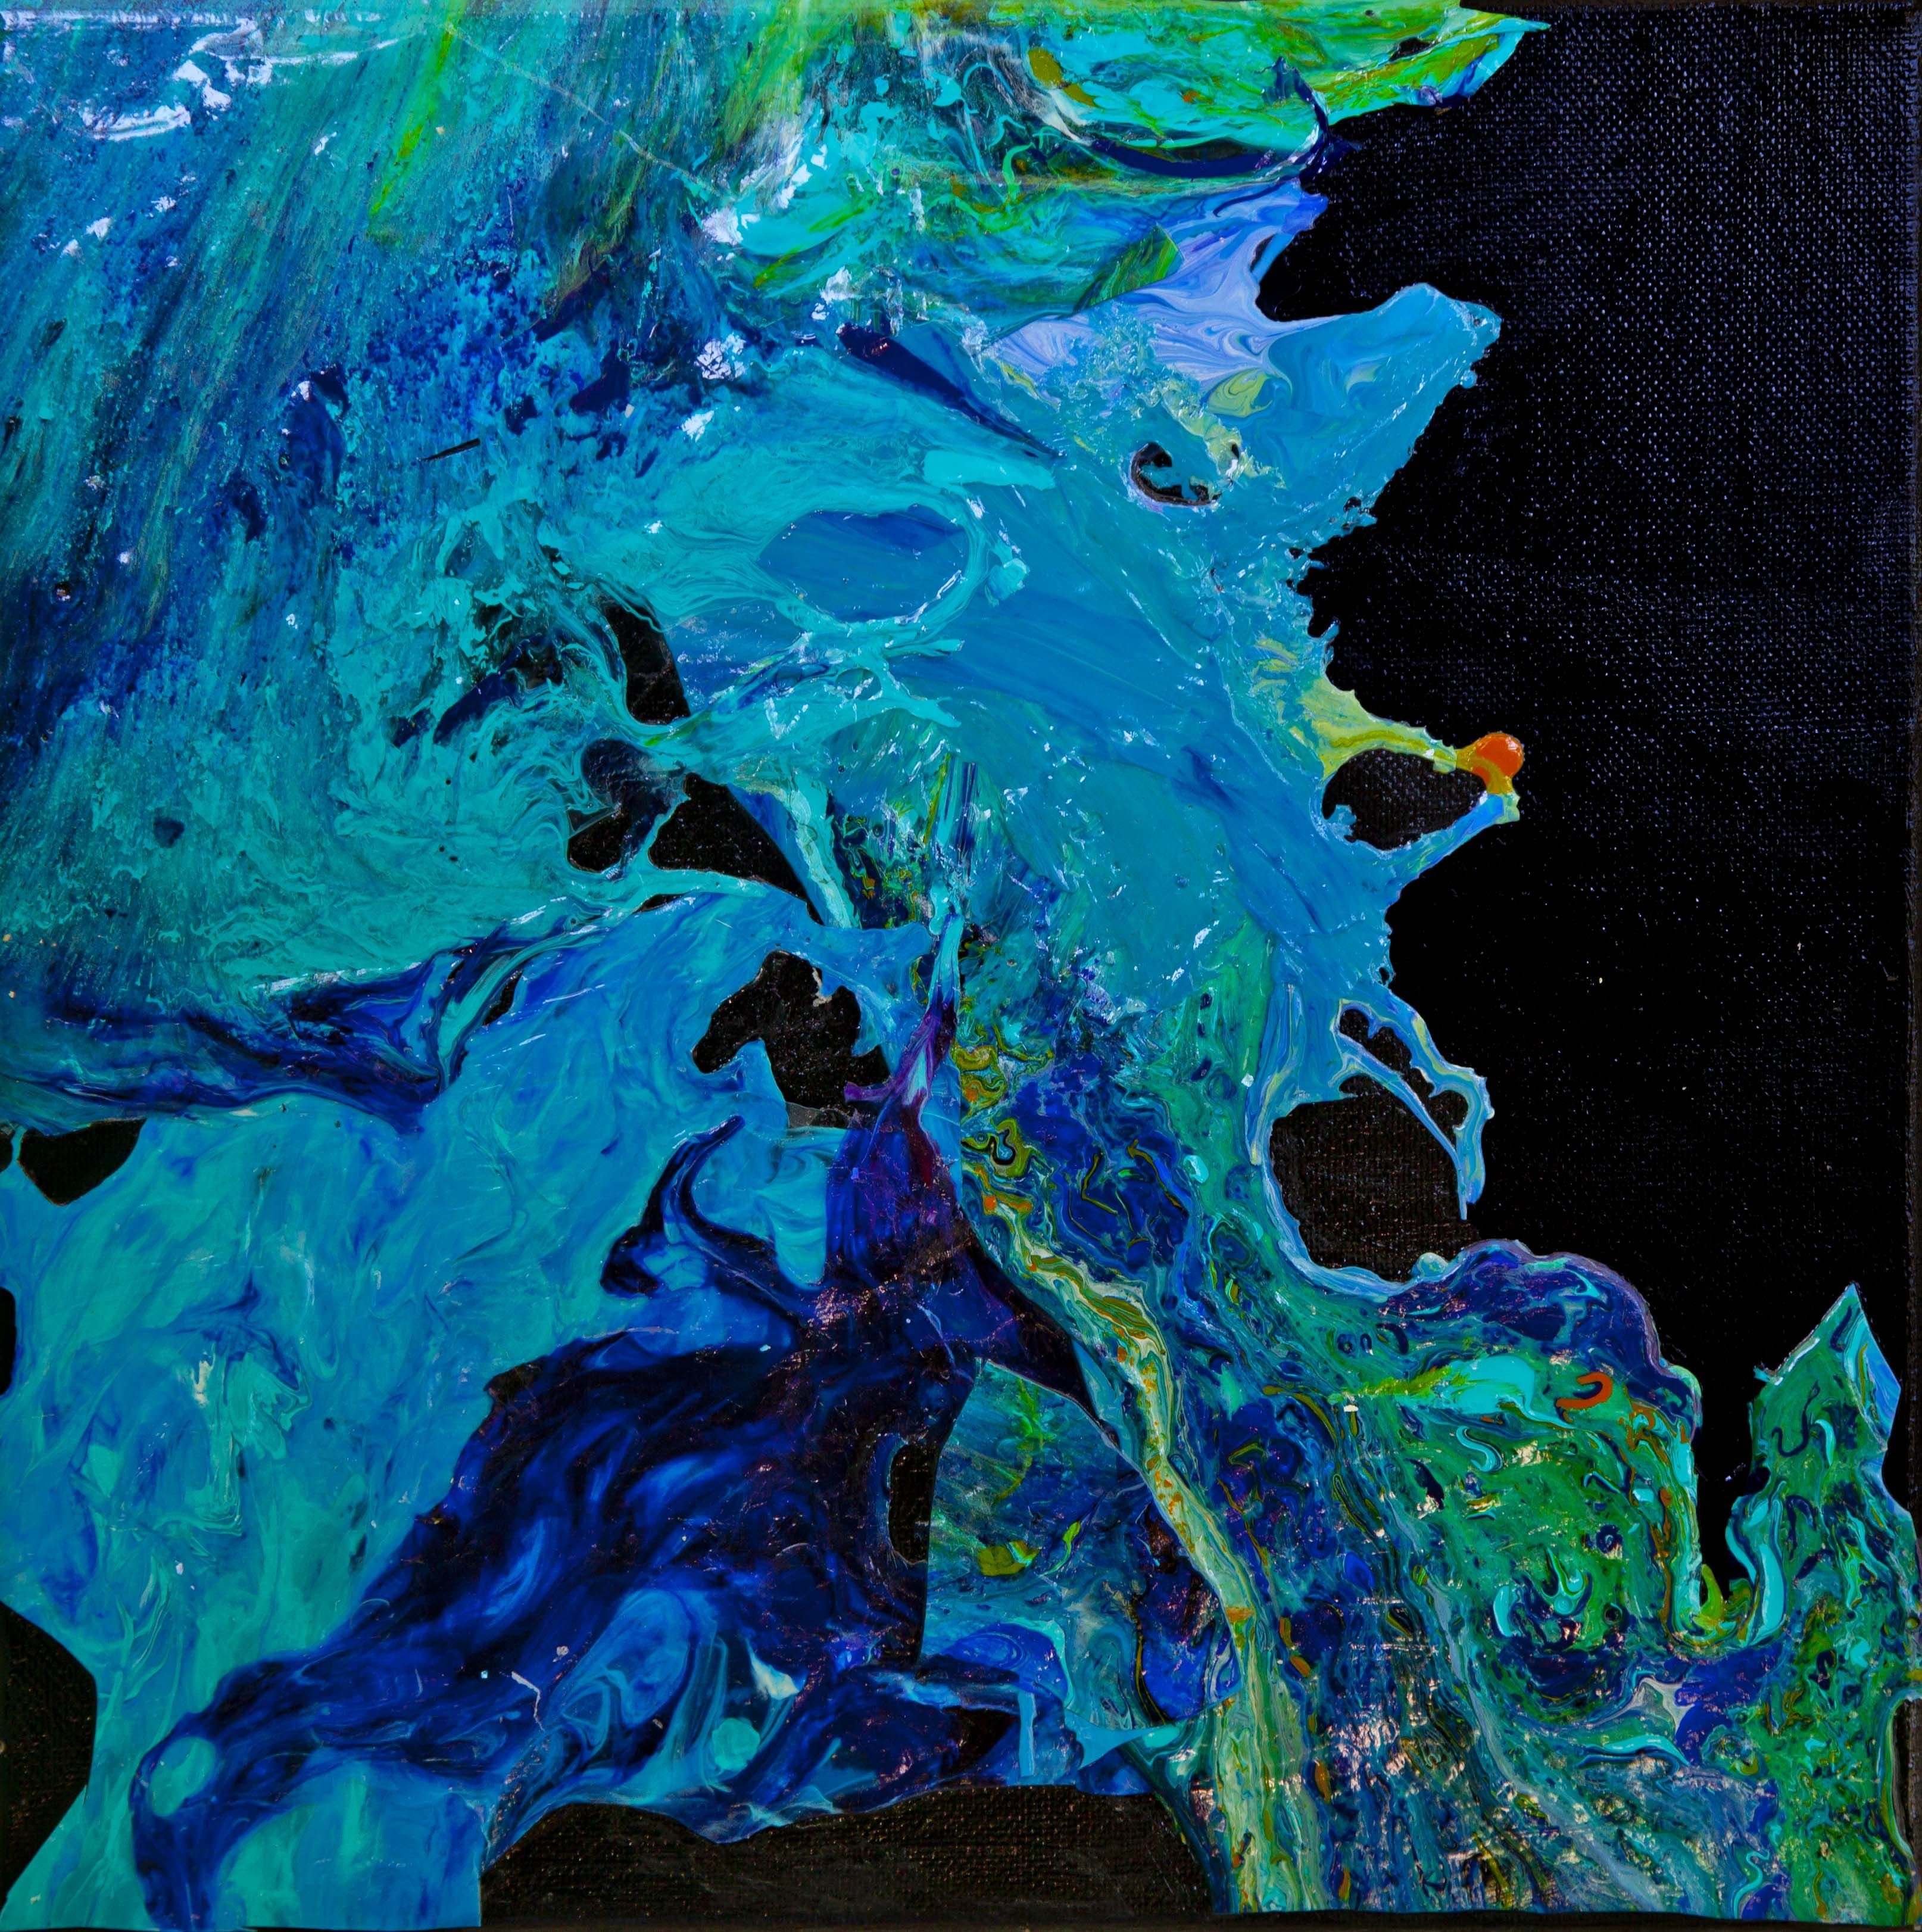
\includegraphics[width=1\linewidth]{graphics/1.jpg}
	%\end{figure}
\end{frame}

\framepic{graphics/1.jpg}{
	\textcolor{ucuwhite}{Thank you!}
 \vskip 0.5cm
 }

\end{document}
